\chapter{Design and implementation}\label{sec:impl}

In order to unroll a loop with non-static bounds this thesis will be following the following approach:
First, we will check whether a loop can be unrolled.
\Cref{sec:impl:unrollability} describes the conditions necessary and how they are checked.
After that, \textit{fixup code}
\footnote{The term \textit{fixup code} describes that code that has to be added to account for cases where the number of times the loop is executed modulo the unrolling factor is not equal to zero.}
,as describe in \cref{sec:impl:fixup}, will be created, and the loop will be unrolled a set number of times and its header will be updated.
The unrolling process will be covered in \cref{sec:impl:unroll}.

In the following a convention will be used, where we will assume loops are like the loop in~\ref{fig:impl:general-loop}.
In \cref{fig:impl:general-loop} \textit{cmp} refers to a comparison that can be one of the following: $<, >, \geq, \leq$.
Further, $I \in \mathbb{Z}$ will refer to the starting value, $N \in \mathbb{Z}$ to the bound, and $c \in \mathbb{Z} \backslash \zeroset$ \label{sec:impl::def-c} to the increment\footnote{N.B.: $c$ may be negative and could hence also be a decrement} of such loop.

\begin{figure}[H]
    \centering
    \begin{algorithmic}
        \Function{Foo}{$I \in \mathbb{Z}, N \in \mathbb{Z}, c \in \mathbb{Z}$}
            \State $i \gets I$
            \While{$i~\text{cmp}~N$}
                \State \Call{DoSomething}{}
                \State $i \gets i + c$
            \EndWhile
        \EndFunction
    \end{algorithmic}
    \caption{A general form of loop starting at $I$ and counting in increments of $c$ up to $N$}
    \label{fig:impl:general-loop}
\end{figure}

\section{Determining unrollability}\label{sec:impl:unrollability}

\section{Unrolling}\label{sec:impl:unroll}

To get started with unrolling loops that have unknown bounds, we will unroll them with a given factor without considering whether the transformation is semantically invariant.
In \cref{sec:impl:fixup} and \cref{sec:impl:preheader} we will be restoring the semantic equivalence.

Since~\libFIRM~already provides an unrolling mechanism for unrolling a loop with a given factor~\cite{aebi18bachelorarbeit}, we will be using it to unroll our loop by a factor $f$.
\Cref{fig:impl:unroll:existing-mechanism} shows a summary of the way the mechanism works.
N.B.: The LCSSA property is preserved across all following operations.

Further, figures~\ref{fig:impl:unroll:unroll-factor-2-before} and,~\ref{fig:impl:unroll:unroll-factor-2-after} show a firm graph of a loop that is to be unrolled or is unrolled using a factor of two, respectively.
Especially to be noted is that in \cref{fig:impl:unroll:unroll-factor-2-after} the loop header is duplicated and that hence the number of conditions did not decrease through the loop unroll.
With the previous usage this was not an issue though, as using a constant bit analysis~\libFIRM~would automatically remove these excess headers~\cite{aebi18bachelorarbeit}.
Unfortunately though in the use cases of an unknown bound that of course does not work, as~\libFIRM~cannot recognize the additional semantics we are adding.
Henceforth, the need to manually prune the graph to remove the excess headers arises.
\Cref{alg:impl:unroll:prune-headers} shows the algorithm used to accomplish this.
First all phis in the header will be rewired, such that all in-loop nodes descending from any given phi node will each get the in-loop predecessesors of the phi node as predecessors themselves, whilst the phi node is no longer a predecessor of any of the descendants.
The same will then be done to the descendants of the block itself.

\begin{algorithm}
    \begin{algorithmic}
        \Function{PruneExcessHeader}{$copiedHeader: \text{Block}$}
            \ForAll{$phi \in copiedHeade$}
                \State \Call{PrunePhi}{$phi, copiedHeader$}
            \EndFor
            \ForAll{$post \in h.descendants$}
                \State $post.predecessors \gets (post.predecessors \backslash \{copiedHeader\}) \cup \newline \{b \vert  b \in copiedHeader.predecessors, b.loop = copiedHeader.loop\}$
            \EndFor
        \EndFunction
        \Function{PrunePhi}{$phi: \text{Phi-Node}, copiedHeader: \text{Block}$}
            \ForAll{$out \in phi.descendants$}
                \Comment $out$ is ensured to be $\phi$ node by the LCSSA construction algorithm~\cite{aebi18bachelorarbeit}
                \If{$out.block \neq copiedHeader$}
                    \State $out.predecessors \gets (out.predecessors \backslash \{phi\}) \cup \newline \{n \vert  n \in phi.predecessors, n.loop = out.loop\}$
                \EndIf
            \EndFor
        \EndFunction
    \end{algorithmic}
    \caption{Pruning excess headers after unrolling}
    \label{alg:impl:unroll:prune-headers}
\end{algorithm}

\begin{algorithm}[h]
    \begin{algorithmic}
        \Function{UnrollExisting}{$factor: \mathbb{N}_{> 1}, loop: \text{Loop}$}
            \State \Call{AssureLCSSA}{$loop$}
            \ForAll{$block \in loop$}
                \For{$i \in \{1..(factor - 1)\}$}
                    \State \Call{DuplicateBlock}{$block$}
                \EndFor
            \EndFor
            \State \Call{RewireDuplicatedBlocks}{} \Comment{Attach blocks to form unrolled structure}
            \State \Comment{$loop$ is still in LCSSA form after unrolling}
        \EndFunction
    \end{algorithmic}
    \caption{Pseudo code for the existing unrolling mechanism~\cite{aebi18bachelorarbeit}}
    \label{fig:impl:unroll:existing-mechanism}
\end{algorithm}

\begin{figure}[H]
    \centering
    \begin{adjustbox}{max width=\textwidth}
        \centering
        % Scale factor 0.024395857307249712
\definecolor{color0}{RGB}{222,239,234}
\definecolor{color1}{RGB}{192,192,192}
\definecolor{color2}{RGB}{153,153,255}
\definecolor{color3}{RGB}{255,153,153}
\definecolor{color4}{RGB}{255,255,255}
\definecolor{color5}{RGB}{255,255,153}
\definecolor{color6}{RGB}{153,255,153}
\definecolor{color7}{RGB}{0,150,60}
\definecolor{color8}{RGB}{170,30,30}
\definecolor{color9}{RGB}{255,0,0}
\definecolor{color10}{RGB}{100,100,255}
\definecolor{color11}{RGB}{0,0,0}
\definecolor{color12}{RGB}{128,0,128}
% Bounding Box: 968.0, 869.0
\begin{tikzpicture}
	\node[fill=color0, draw, minimum width=17.40644418872267cm, minimum height=8.611737629459148cm] (n1) at (14.895584286649068cm ,-2.427387802071346cm) {};
	% 1 node layouts
	\node[scale=0.8871220838999895, transform shape] at (14.895584286649068cm ,1.599834579976985cm) {Block  227};
	\node[fill=color0, draw, minimum width=9.73825221688215cm, minimum height=8.855696202531645cm] (n2) at (5.601001827658567cm ,7.282163406214039cm) {};
	% 1 node layouts
	\node[scale=0.8871220838999895, transform shape] at (5.601001827658567cm ,11.431365074798618cm) {Block  217};
	\node[fill=color1, draw, minimum width=23.5988063810104cm, minimum height=21.2cm] (n3) at (12.165341050113947cm ,3.5008055235903335cm) {};
	% 1 node layouts
	\node[scale=0.8871220838999895, transform shape] at (12.165341050113947cm ,13.822159090909091cm) {\#LOOP-6};
	\node[fill=color2, draw, minimum width=2.342002301495972cm, minimum height=0.7318757192174914cm] (n4) at (2.312583767684289cm ,8.709321058688147cm) {};
	% 1 node layouts
	\node[scale=0.8871220838999895, transform shape] at (2.312583767684289cm ,8.709321058688147cm) {Phi[loop]  218};
	\node[fill=color3, draw, minimum width=2.634752589182969cm, minimum height=0.7318757192174914cm] (n5) at (5.761727475800447cm ,3.5861910241657076cm) {};
	% 1 node layouts
	\node[scale=0.8871220838999895, transform shape] at (5.761727475800447cm ,3.5861910241657076cm) {Proj X false 226};
	\node[fill=color3, draw, minimum width=2.53716915995397cm, minimum height=0.7318757192174914cm] (n6) at (8.83560549651391cm ,3.5861910241657076cm) {};
	% 1 node layouts
	\node[scale=0.8871220838999895, transform shape] at (8.83560549651391cm ,3.5861910241657076cm) {Proj X true 225};
	\node[fill=color3, draw, minimum width=1.854085155350978cm, minimum height=0.7318757192174914cm] (n7) at (7.264942801055981cm ,5.293901035673187cm) {};
	% 1 node layouts
	\node[scale=0.8871220838999895, transform shape] at (7.264942801055981cm ,5.293901035673187cm) {Cond  224};
	\node[fill=color4, draw, minimum width=3.5373993095512084cm, minimum height=0.7318757192174914cm] (n8) at (7.264942801055981cm ,7.001611047180667cm) {};
	% 1 node layouts
	\node[scale=0.8871220838999895, transform shape] at (7.264942801055981cm ,7.001611047180667cm) {Cmp b less\_equal 223};
	\node[fill=color5, draw, minimum width=2.9762945914844647cm, minimum height=0.7318757192174914cm] (n9) at (8.149292628443783cm ,8.709321058688147cm) {};
	% 1 node layouts
	\node[scale=0.8871220838999895, transform shape] at (8.149292628443783cm ,8.709321058688147cm) {Const 0x10 Is 222};
	\node[fill=color6, draw, minimum width=1.7565017261219793cm, minimum height=0.7318757192174914cm] (n10) at (5.20349285859338cm ,8.709321058688147cm) {};
	% 1 node layouts
	\node[scale=0.8871220838999895, transform shape] at (5.20349285859338cm ,8.709321058688147cm) {Phi Is 219};
	\node[fill=color5, draw, minimum width=2.781127733026467cm, minimum height=0.7318757192174914cm] (n11) at (6.2984363365599405cm ,10.417031070195627cm) {};
	% 1 node layouts
	\node[scale=0.8871220838999895, transform shape] at (6.2984363365599405cm ,10.417031070195627cm) {Const 0x0 Is 215};
	\node[fill=color7, draw, minimum width=0.48791714614499426cm, minimum height=0.48791714614499426cm] (n12) at (1.3417721518987342cm ,7.001611047180667cm) {};
	\node[fill=color7, draw, minimum width=0.48791714614499426cm, minimum height=0.48791714614499426cm] (n13) at (4.7643674270628855cm ,7.001611047180667cm) {};
	\node[fill=color7, draw, minimum width=0.48791714614499426cm, minimum height=0.48791714614499426cm] (n14) at (2.8005009138292833cm ,10.417031070195627cm) {};
	\node[fill=color7, draw, minimum width=0.48791714614499426cm, minimum height=0.48791714614499426cm] (n15) at (1.824666621539295cm ,10.417031070195627cm) {};
	\node[fill=color7, draw, minimum width=0.48791714614499426cm, minimum height=0.48791714614499426cm] (n16) at (4.175996750829215cm ,10.417031070195627cm) {};
	\node[fill=color7, draw, minimum width=0.48791714614499426cm, minimum height=0.48791714614499426cm] (n17) at (2.3176064441887227cm ,7.001611047180667cm) {};
	\node[fill=color7, draw, minimum width=0.48791714614499426cm, minimum height=0.48791714614499426cm] (n18) at (3.297745887768226cm ,7.001611047180667cm) {};
	\node[fill=color2, draw, minimum width=2.268814729574223cm, minimum height=0.7318757192174914cm] (n19) at (13.047598095624902cm ,-4.537629459148446cm) {};
	% 1 node layouts
	\node[scale=0.8871220838999895, transform shape] at (13.047598095624902cm ,-4.537629459148446cm) {Proj M M 235};
	\node[fill=color2, draw, minimum width=1.6345224395857307cm, minimum height=0.7318757192174914cm] (n20) at (13.047598095624902cm ,-2.8299194476409664cm) {};
	% 1 node layouts
	\node[scale=0.8871220838999895, transform shape] at (13.047598095624902cm ,-2.8299194476409664cm) {Call  234};
	\node[fill=color5, draw, minimum width=3.659378596087457cm, minimum height=0.7318757192174914cm] (n21) at (9.961522146257813cm ,-1.1222094361334867cm) {};
	% 1 node layouts
	\node[scale=0.8871220838999895, transform shape] at (9.961522146257813cm ,-1.1222094361334867cm) {Address \&\_printf P 229};
	\node[fill=color5, draw, minimum width=3.41542002301496cm, minimum height=0.7318757192174914cm] (n22) at (16.011694758455743cm ,-1.1222094361334867cm) {};
	% 1 node layouts
	\node[scale=0.8871220838999895, transform shape] at (16.011694758455743cm ,-1.1222094361334867cm) {Address \&str.0 P 233};
	\node[fill=color2, draw, minimum width=1.5369390103567317cm, minimum height=0.7318757192174914cm] (n23) at (13.047598095624902cm ,-1.1222094361334867cm) {};
	% 1 node layouts
	\node[scale=0.8871220838999895, transform shape] at (13.047598095624902cm ,-1.1222094361334867cm) {Phi  403};
	\node[fill=color3, draw, minimum width=1.6833141542002301cm, minimum height=0.7318757192174914cm] (n24) at (7.3999571289965935cm ,0.585500575373993cm) {};
	% 1 node layouts
	\node[scale=0.8871220838999895, transform shape] at (7.3999571289965935cm ,0.585500575373993cm) {Jmp  240};
	\node[fill=color4, draw, minimum width=1.9272727272727272cm, minimum height=0.7318757192174914cm] (n25) at (20.477007926300555cm ,-2.8299194476409664cm) {};
	% 1 node layouts
	\node[scale=0.8871220838999895, transform shape] at (20.477007926300555cm ,-2.8299194476409664cm) {Add Is 239};
	\node[fill=color5, draw, minimum width=2.781127733026467cm, minimum height=0.7318757192174914cm] (n26) at (21.842304654888423cm ,-1.1222094361334867cm) {};
	% 1 node layouts
	\node[scale=0.8871220838999895, transform shape] at (21.842304654888423cm ,-1.1222094361334867cm) {Const 0x1 Is 238};
	\node[fill=color6, draw, minimum width=1.7565017261219793cm, minimum height=0.7318757192174914cm] (n27) at (19.085572779169205cm ,-1.1222094361334867cm) {};
	% 1 node layouts
	\node[scale=0.8871220838999895, transform shape] at (19.085572779169205cm ,-1.1222094361334867cm) {Phi Is 402};
	\node[fill=color7, draw, minimum width=0.48791714614499426cm, minimum height=0.48791714614499426cm] (n28) at (13.047598095624902cm ,0.585500575373993cm) {};
	\node[fill=color7, draw, minimum width=0.48791714614499426cm, minimum height=0.48791714614499426cm] (n29) at (19.085572779169205cm ,0.585500575373993cm) {};
	\node[fill=color7, draw, minimum width=0.48791714614499426cm, minimum height=0.48791714614499426cm] (n30) at (13.047598095624902cm ,-6.123360184119678cm) {};
	\node[fill=color7, draw, minimum width=0.48791714614499426cm, minimum height=0.48791714614499426cm] (n31) at (20.477007926300555cm ,-4.537629459148446cm) {};
	\node[fill=color8, draw, minimum width=0.48791714614499426cm, minimum height=0.48791714614499426cm] (n32) at (5.1228908594508cm ,12.929804372842348cm) {};
	\node[fill=color8, draw, minimum width=0.48791714614499426cm, minimum height=0.48791714614499426cm] (n33) at (7.3999571289965935cm ,-1.1222094361334867cm) {};
	\draw[color=color9, -latex] (14.895584286649068cm ,1.8784810126582279cm) -- (14.895584286649068cm ,2.366398158803222cm) -- (8.83560549651391cm ,2.366398158803222cm) -- (8.83560549651391cm ,3.220253164556962cm);
	\node[] at (15.090751145107065cm ,2.2337456846950516cm) {
		\scalebox{0.8871220838999895}{0}
	};
	\draw[color=color10, -latex] (2.8980843430582826cm ,9.075258918296893cm) -- (2.8980843430582826cm ,9.563176064441887cm) -- (2.8005009138292833cm ,9.563176064441887cm) -- (2.8005009138292833cm ,10.17307249712313cm);
	\node[] at (3.09325120151628cm ,9.430523590333717cm) {
		\scalebox{0.8871220838999895}{0}
	};
	\draw[color=color10, -latex] (1.7270831923102963cm ,9.075258918296893cm) -- (1.7270831923102963cm ,9.563176064441887cm) -- (1.824666621539295cm ,9.563176064441887cm) -- (1.824666621539295cm ,10.17307249712313cm);
	\node[] at (1.9222500507682938cm ,9.430523590333717cm) {
		\scalebox{0.8871220838999895}{1}
	};
	\draw[color=color9, -latex] (5.761727475800447cm ,3.9521288837744533cm) -- (5.761727475800447cm ,4.440046029919448cm) -- (6.801421512218236cm ,4.440046029919448cm) -- (6.801421512218236cm ,4.927963176064441cm);
	\node[] at (5.956894334258444cm ,4.307393555811277cm) {
		\scalebox{0.8871220838999895}{0}
	};
	\draw[color=color9, -latex] (8.83560549651391cm ,3.9521288837744533cm) -- (8.83560549651391cm ,4.440046029919448cm) -- (7.728464089893725cm ,4.440046029919448cm) -- (7.728464089893725cm ,4.927963176064441cm);
	\node[] at (9.030772354971909cm ,4.307393555811277cm) {
		\scalebox{0.8871220838999895}{0}
	};
	\draw[color=color11, -latex] (7.264942801055981cm ,5.659838895281933cm) -- (7.264942801055981cm ,6.635673187571921cm);
	\node[] at (7.460109659513979cm ,6.128029703682393cm) {
		\scalebox{0.8871220838999895}{0}
	};
	\draw[color=color11, -latex] (6.380592973668179cm ,7.367548906789413cm) -- (6.380592973668179cm ,7.855466052934407cm) -- (5.642618290123875cm ,7.855466052934407cm) -- (5.642618290123875cm ,8.343383199079401cm);
	\node[] at (6.5757598321261765cm ,7.722813578826237cm) {
		\scalebox{0.8871220838999895}{0}
	};
	\draw[color=color11, -latex] (8.149292628443783cm ,7.367548906789413cm) -- (8.149292628443783cm ,8.343383199079401cm);
	\node[] at (8.34445948690178cm ,7.835739715189873cm) {
		\scalebox{0.8871220838999895}{1}
	};
	\draw[color=color11, -latex] (5.642618290123875cm ,9.075258918296893cm) -- (5.642618290123875cm ,9.563176064441887cm) -- (6.2984363365599405cm ,9.563176064441887cm) -- (6.2984363365599405cm ,10.051093210586881cm);
	\node[] at (5.837785148581872cm ,9.430523590333717cm) {
		\scalebox{0.8871220838999895}{0}
	};
	\draw[color=color11, -latex] (4.7643674270628855cm ,9.075258918296893cm) -- (4.7643674270628855cm ,9.563176064441887cm) -- (4.175996750829215cm ,9.563176064441887cm) -- (4.175996750829215cm ,10.17307249712313cm);
	\node[] at (4.959534285520883cm ,9.430523590333717cm) {
		\scalebox{0.8871220838999895}{1}
	};
	\draw[color=color10, -latex] (1.3417721518987342cm ,7.245569620253164cm) -- (1.3417721518987342cm ,7.855466052934407cm) -- (1.5319163338522985cm ,7.855466052934407cm) -- (1.5319163338522985cm ,8.343383199079401cm);
	\node[] at (1.5369390103567317cm ,7.661823935558113cm) {
		\scalebox{0.8871220838999895}{0}
	};
	\draw[color=color11, -latex] (4.7643674270628855cm ,7.245569620253164cm) -- (4.7643674270628855cm ,8.343383199079401cm);
	\node[] at (4.959534285520883cm ,7.713760428653624cm) {
		\scalebox{0.8871220838999895}{0}
	};
	\draw[color=color10, -latex] (2.3176064441887227cm ,7.245569620253164cm) -- (2.312583767684289cm ,8.343383199079401cm);
	\node[] at (2.5116432004332228cm ,7.713760428653624cm) {
		\scalebox{0.8871220838999895}{0}
	};
	\draw[color=color12, -latex] (3.297745887768226cm ,7.245569620253164cm) -- (3.297745887768226cm ,7.855466052934407cm) -- (3.09325120151628cm ,7.855466052934407cm) -- (3.09325120151628cm ,8.343383199079401cm);
	\node[] at (3.4929127462262235cm ,7.661823935558113cm) {
		\scalebox{0.8871220838999895}{1}
	};
	\draw[color=color10, -latex] (13.047598095624902cm ,-4.171691599539701cm) -- (13.047598095624902cm ,-3.195857307249712cm);
	\node[] at (13.242764954082899cm ,-3.7035007911392404cm) {
		\scalebox{0.8871220838999895}{0}
	};
	\draw[color=color10, -latex] (13.047598095624902cm ,-2.4639815880322207cm) -- (13.047598095624902cm ,-1.4881472957422324cm);
	\node[] at (13.242764954082899cm ,-1.9957907796317607cm) {
		\scalebox{0.8871220838999895}{0}
	};
	\draw[color=color11, -latex] (12.502757282429657cm ,-2.4639815880322207cm) -- (12.502757282429657cm ,-1.9760644418872266cm) -- (9.961522146257813cm ,-1.9760644418872266cm) -- (9.961522146257813cm ,-1.4881472957422324cm);
	\node[] at (12.697924140887656cm ,-2.108716915995397cm) {
		\scalebox{0.8871220838999895}{1}
	};
	\draw[color=color11, -latex] (13.592438908820146cm ,-2.4639815880322207cm) -- (13.592438908820144cm ,-1.9760644418872266cm) -- (16.011694758455743cm ,-1.9760644418872266cm) -- (16.011694758455743cm ,-1.4881472957422324cm);
	\node[] at (13.787605767278144cm ,-2.108716915995397cm) {
		\scalebox{0.8871220838999895}{2}
	};
	\draw[color=color10, -latex] (13.047598095624902cm ,-0.7562715765247411cm) -- (13.047598095624902cm ,0.34154200230149595cm);
	\node[] at (13.242764954082899cm ,-0.2880807681242808cm) {
		\scalebox{0.8871220838999895}{0}
	};
	\draw[color=color11, -latex] (19.99518974448237cm ,-2.4639815880322207cm) -- (19.99518974448237cm ,-1.9760644418872266cm) -- (19.085572779169205cm ,-1.9760644418872266cm) -- (19.085572779169205cm ,-1.4881472957422324cm);
	\node[] at (20.19035660294037cm ,-2.108716915995397cm) {
		\scalebox{0.8871220838999895}{0}
	};
	\draw[color=color11, -latex] (20.958826108118735cm ,-2.4639815880322207cm) -- (20.958826108118735cm ,-1.9760644418872266cm) -- (21.842304654888423cm ,-1.9760644418872266cm) -- (21.842304654888423cm ,-1.4881472957422324cm);
	\node[] at (21.153992966576734cm ,-2.108716915995397cm) {
		\scalebox{0.8871220838999895}{1}
	};
	\draw[color=color11, -latex] (19.085572779169205cm ,-0.7562715765247411cm) -- (19.085572779169205cm ,0.34154200230149595cm);
	\node[] at (19.280739637627203cm ,-0.2880807681242808cm) {
		\scalebox{0.8871220838999895}{0}
	};
	\draw[color=color10, -latex] (13.047598095624902cm ,-5.8794016110471805cm) -- (13.047598095624902cm ,-4.903567318757192cm);
	\node[] at (13.242764954082899cm ,-5.41121080264672cm) {
		\scalebox{0.8871220838999895}{1}
	};
	\draw[color=color11, -latex] (20.477007926300555cm ,-4.293670886075949cm) -- (20.477007926300555cm ,-3.195857307249712cm);
	\node[] at (20.67217478475855cm ,-3.825480077675489cm) {
		\scalebox{0.8871220838999895}{1}
	};
	\draw[color=color9, -latex] (8.035564881879104cm ,11.710011507479862cm) -- (8.035564881879104cm ,12.197928653624857cm) -- (5.1228908594508cm ,12.197928653624857cm) -- (5.1228908594508cm ,12.68584579976985cm);
	\node[] at (8.2307317403371cm ,12.065276179516685cm) {
		\scalebox{0.8871220838999895}{1}
	};
	\draw[color=color9, -latex] (7.3999571289965935cm ,-0.8782508630609897cm) -- (7.3999571289965935cm ,0.2195627157652474cm);
	\node[] at (7.595123987454591cm ,-0.41006005466052936cm) {
		\scalebox{0.8871220838999895}{1}
	};
\end{tikzpicture}

    \end{adjustbox}
    \caption{Firm graph of a loop with an unknown bound}
    \label{fig:impl:unroll:unroll-factor-2-before}
\end{figure}
\begin{figure}[h]
    \centering
    \begin{adjustbox}{max width=\textwidth}
        \centering
        % Scale factor 0.012809667673716012
\definecolor{color13}{RGB}{222,239,234}
\definecolor{color14}{RGB}{192,192,192}
\definecolor{color15}{RGB}{153,153,255}
\definecolor{color16}{RGB}{255,255,153}
\definecolor{color17}{RGB}{255,153,153}
\definecolor{color18}{RGB}{255,255,255}
\definecolor{color19}{RGB}{153,255,153}
\definecolor{color20}{RGB}{0,150,60}
\definecolor{color21}{RGB}{170,30,30}
\definecolor{color22}{RGB}{255,0,0}
\definecolor{color23}{RGB}{100,100,255}
\definecolor{color24}{RGB}{0,0,0}
\definecolor{color25}{RGB}{128,0,128}
% Bounding Box: 1325.0, 1655.0
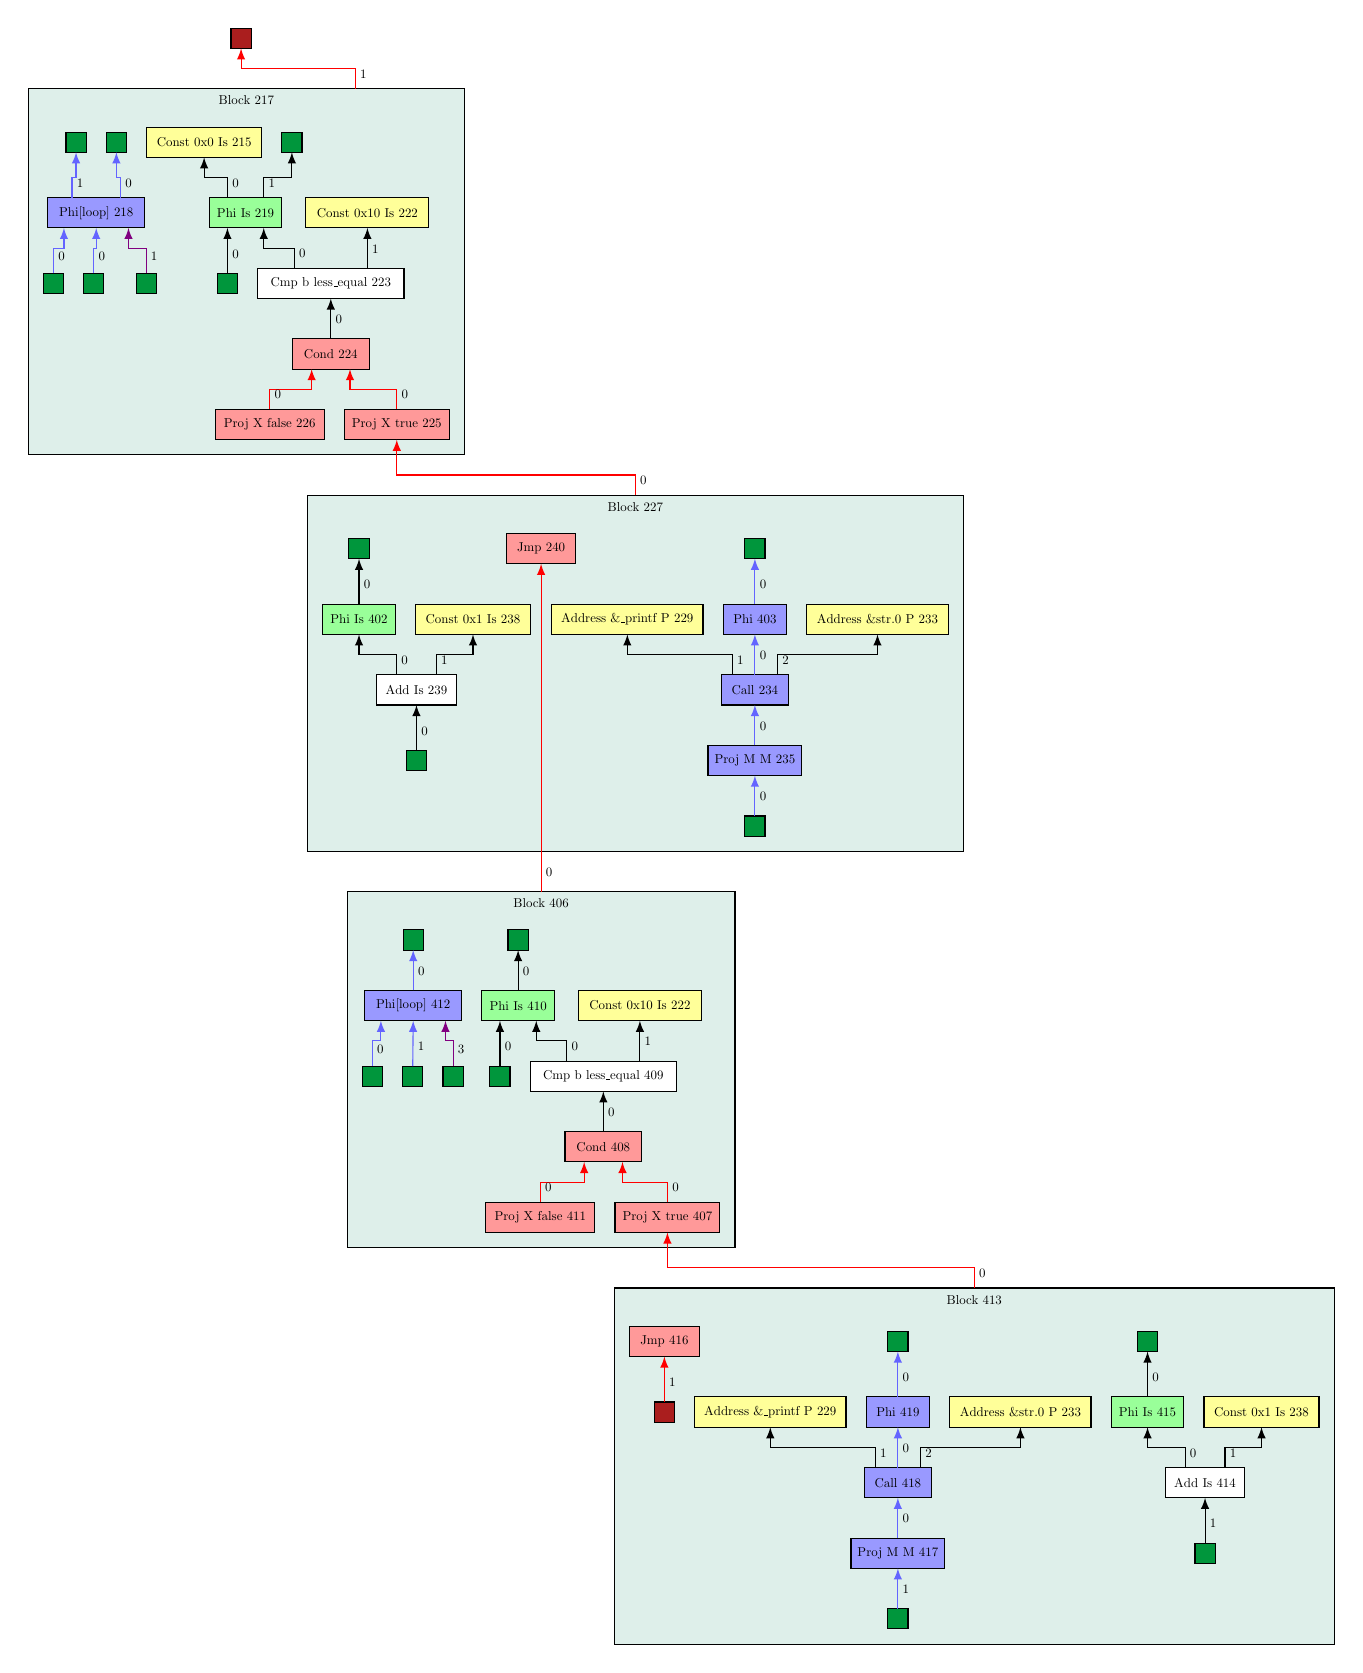
\begin{tikzpicture}
	\node[fill=color13, draw, minimum width=9.139697885196375cm, minimum height=4.521812688821752cm] (n34) at (12.39926257798397cm ,-1.2745619335347431cm) {};
	% 1 node layouts
	\node[scale=0.4658060972260368, transform shape] at (12.39926257798397cm ,0.8400339879154078cm) {Block  413};
	\node[fill=color13, draw, minimum width=5.539051004087435cm, minimum height=4.649909365558912cm] (n35) at (3.153815532255198cm ,13.892084592145014cm) {};
	% 1 node layouts
	\node[scale=0.4658060972260368, transform shape] at (3.153815532255198cm ,16.070728851963747cm) {Block  217};
	\node[fill=color13, draw, minimum width=8.326283987915408cm, minimum height=4.521812688821752cm] (n36) at (8.09521423961539cm ,8.793836858006042cm) {};
	% 1 node layouts
	\node[scale=0.4658060972260368, transform shape] at (8.09521423961539cm ,10.908432779456193cm) {Block  227};
	\node[fill=color13, draw, minimum width=4.925317220543807cm, minimum height=4.521812688821752cm] (n37) at (6.897510312122942cm ,3.7596374622356494cm) {};
	% 1 node layouts
	\node[scale=0.4658060972260368, transform shape] at (6.897510312122942cm ,5.874233383685801cm) {Block  406};
	% 1 node layouts
	\node[fill=color15, draw, minimum width=1.1912990936555892cm, minimum height=0.38429003021148034cm] (n39) at (9.613159858950738cm ,7.685800604229607cm) {};
	% 1 node layouts
	\node[scale=0.4658060972260368, transform shape] at (9.613159858950738cm ,7.685800604229607cm) {Proj M M 235};
	\node[fill=color15, draw, minimum width=0.8582477341389728cm, minimum height=0.38429003021148034cm] (n40) at (9.613159858950738cm ,8.582477341389728cm) {};
	% 1 node layouts
	\node[scale=0.4658060972260368, transform shape] at (9.613159858950738cm ,8.582477341389728cm) {Call  234};
	\node[fill=color16, draw, minimum width=1.9214501510574018cm, minimum height=0.38429003021148034cm] (n41) at (7.992736898225662cm ,9.479154078549849cm) {};
	% 1 node layouts
	\node[scale=0.4658060972260368, transform shape] at (7.992736898225662cm ,9.479154078549849cm) {Address \&\_printf P 229};
	\node[fill=color16, draw, minimum width=1.7933534743202417cm, minimum height=0.38429003021148034cm] (n42) at (11.169534481307233cm ,9.479154078549849cm) {};
	% 1 node layouts
	\node[scale=0.4658060972260368, transform shape] at (11.169534481307233cm ,9.479154078549849cm) {Address \&str.0 P 233};
	\node[fill=color15, draw, minimum width=0.8070090634441087cm, minimum height=0.38429003021148034cm] (n43) at (9.613159858950738cm ,9.479154078549849cm) {};
	% 1 node layouts
	\node[scale=0.4658060972260368, transform shape] at (9.613159858950738cm ,9.479154078549849cm) {Phi  403};
	\node[fill=color17, draw, minimum width=0.8838670694864048cm, minimum height=0.38429003021148034cm] (n44) at (6.897510312122942cm ,10.37583081570997cm) {};
	% 1 node layouts
	\node[scale=0.4658060972260368, transform shape] at (6.897510312122942cm ,10.37583081570997cm) {Jmp  240};
	\node[fill=color18, draw, minimum width=1.0119637462235649cm, minimum height=0.38429003021148034cm] (n45) at (5.314448882112871cm ,8.582477341389728cm) {};
	% 1 node layouts
	\node[scale=0.4658060972260368, transform shape] at (5.314448882112871cm ,8.582477341389728cm) {Add Is 239};
	\node[fill=color16, draw, minimum width=1.4603021148036255cm, minimum height=0.38429003021148034cm] (n46) at (6.032857744147112cm ,9.479154078549849cm) {};
	% 1 node layouts
	\node[scale=0.4658060972260368, transform shape] at (6.032857744147112cm ,9.479154078549849cm) {Const 0x1 Is 238};
	\node[fill=color19, draw, minimum width=0.9222960725075529cm, minimum height=0.38429003021148034cm] (n47) at (4.585365297017201cm ,9.479154078549849cm) {};
	% 1 node layouts
	\node[scale=0.4658060972260368, transform shape] at (4.585365297017201cm ,9.479154078549849cm) {Phi Is 402};
	\node[fill=color20, draw, minimum width=0.25619335347432026cm, minimum height=0.25619335347432026cm] (n48) at (9.613159858950738cm ,10.37583081570997cm) {};
	\node[fill=color20, draw, minimum width=0.25619335347432026cm, minimum height=0.25619335347432026cm] (n49) at (4.585365297017202cm ,10.37583081570997cm) {};
	\node[fill=color20, draw, minimum width=0.25619335347432026cm, minimum height=0.25619335347432026cm] (n50) at (9.613159858950738cm ,6.853172205438066cm) {};
	\node[fill=color20, draw, minimum width=0.25619335347432026cm, minimum height=0.25619335347432026cm] (n51) at (5.314448882112871cm ,7.685800604229607cm) {};
	\node[fill=color15, draw, minimum width=1.1912990936555892cm, minimum height=0.38429003021148034cm] (n52) at (11.428930251699981cm ,-2.3825981873111783cm) {};
	% 1 node layouts
	\node[scale=0.4658060972260368, transform shape] at (11.428930251699981cm ,-2.3825981873111783cm) {Proj M M 417};
	\node[fill=color15, draw, minimum width=0.8582477341389728cm, minimum height=0.38429003021148034cm] (n53) at (11.428930251699981cm ,-1.4859214501510574cm) {};
	% 1 node layouts
	\node[scale=0.4658060972260368, transform shape] at (11.428930251699981cm ,-1.4859214501510574cm) {Call  418};
	\node[fill=color16, draw, minimum width=1.9214501510574018cm, minimum height=0.38429003021148034cm] (n54) at (9.808507290974907cm ,-0.5892447129909365cm) {};
	% 1 node layouts
	\node[scale=0.4658060972260368, transform shape] at (9.808507290974907cm ,-0.5892447129909365cm) {Address \&\_printf P 229};
	\node[fill=color16, draw, minimum width=1.7933534743202417cm, minimum height=0.38429003021148034cm] (n55) at (12.985304874056476cm ,-0.5892447129909365cm) {};
	% 1 node layouts
	\node[scale=0.4658060972260368, transform shape] at (12.985304874056476cm ,-0.5892447129909365cm) {Address \&str.0 P 233};
	\node[fill=color15, draw, minimum width=0.8070090634441087cm, minimum height=0.38429003021148034cm] (n56) at (11.428930251699981cm ,-0.5892447129909365cm) {};
	% 1 node layouts
	\node[scale=0.4658060972260368, transform shape] at (11.428930251699981cm ,-0.5892447129909365cm) {Phi  419};
	\node[fill=color17, draw, minimum width=0.8838670694864048cm, minimum height=0.38429003021148034cm] (n57) at (8.463492185234724cm ,0.3074320241691843cm) {};
	% 1 node layouts
	\node[scale=0.4658060972260368, transform shape] at (8.463492185234724cm ,0.3074320241691843cm) {Jmp  416};
	\node[fill=color18, draw, minimum width=1.0119637462235649cm, minimum height=0.38429003021148034cm] (n58) at (15.329931546477708cm ,-1.4859214501510574cm) {};
	% 1 node layouts
	\node[scale=0.4658060972260368, transform shape] at (15.329931546477708cm ,-1.4859214501510574cm) {Add Is 414};
	\node[fill=color16, draw, minimum width=1.4603021148036255cm, minimum height=0.38429003021148034cm] (n59) at (16.0468154480746cm ,-0.5892447129909365cm) {};
	% 1 node layouts
	\node[scale=0.4658060972260368, transform shape] at (16.0468154480746cm ,-0.5892447129909365cm) {Const 0x1 Is 238};
	\node[fill=color19, draw, minimum width=0.9222960725075529cm, minimum height=0.38429003021148034cm] (n60) at (14.599323000944695cm ,-0.5892447129909365cm) {};
	% 1 node layouts
	\node[scale=0.4658060972260368, transform shape] at (14.599323000944695cm ,-0.5892447129909365cm) {Phi Is 415};
	\node[fill=color20, draw, minimum width=0.25619335347432026cm, minimum height=0.25619335347432026cm] (n61) at (11.428930251699981cm ,0.3074320241691843cm) {};
	\node[fill=color20, draw, minimum width=0.25619335347432026cm, minimum height=0.25619335347432026cm] (n62) at (14.599323000944695cm ,0.3074320241691843cm) {};
	\node[fill=color20, draw, minimum width=0.25619335347432026cm, minimum height=0.25619335347432026cm] (n63) at (11.428930251699981cm ,-3.215226586102719cm) {};
	\node[fill=color20, draw, minimum width=0.25619335347432026cm, minimum height=0.25619335347432026cm] (n64) at (15.329931546477708cm ,-2.3825981873111783cm) {};
	\node[fill=color15, draw, minimum width=1.2297280966767372cm, minimum height=0.38429003021148034cm] (n65) at (5.27345794555698cm ,4.573051359516616cm) {};
	% 1 node layouts
	\node[scale=0.4658060972260368, transform shape] at (5.27345794555698cm ,4.573051359516616cm) {Phi[loop]  412};
	\node[fill=color17, draw, minimum width=1.3834441087613294cm, minimum height=0.38429003021148034cm] (n66) at (6.8879030613676555cm ,1.8830211480362538cm) {};
	% 1 node layouts
	\node[scale=0.4658060972260368, transform shape] at (6.8879030613676555cm ,1.8830211480362538cm) {Proj X false 411};
	\node[fill=color17, draw, minimum width=1.3322054380664652cm, minimum height=0.38429003021148034cm] (n67) at (8.501921188255873cm ,1.8830211480362538cm) {};
	% 1 node layouts
	\node[scale=0.4658060972260368, transform shape] at (8.501921188255873cm ,1.8830211480362538cm) {Proj X true 407};
	\node[fill=color17, draw, minimum width=0.973534743202417cm, minimum height=0.38429003021148034cm] (n68) at (7.688080302052448cm ,2.7796978851963745cm) {};
	% 1 node layouts
	\node[scale=0.4658060972260368, transform shape] at (7.688080302052448cm ,2.7796978851963745cm) {Cond  408};
	\node[fill=color18, draw, minimum width=1.8574018126888217cm, minimum height=0.38429003021148034cm] (n69) at (7.688080302052448cm ,3.6763746223564953cm) {};
	% 1 node layouts
	\node[scale=0.4658060972260368, transform shape] at (7.688080302052448cm ,3.6763746223564953cm) {Cmp b less\_equal 409};
	\node[fill=color16, draw, minimum width=1.5627794561933535cm, minimum height=0.38429003021148034cm] (n70) at (8.152430755224653cm ,4.573051359516616cm) {};
	% 1 node layouts
	\node[scale=0.4658060972260368, transform shape] at (8.152430755224653cm ,4.573051359516616cm) {Const 0x10 Is 222};
	\node[fill=color19, draw, minimum width=0.9222960725075529cm, minimum height=0.38429003021148034cm] (n71) at (6.605663383623445cm ,4.573051359516616cm) {};
	% 1 node layouts
	\node[scale=0.4658060972260368, transform shape] at (6.605663383623445cm ,4.573051359516616cm) {Phi Is 410};
	\node[fill=color20, draw, minimum width=0.25619335347432026cm, minimum height=0.25619335347432026cm] (n72) at (4.755093393693938cm ,3.6763746223564953cm) {};
	\node[fill=color20, draw, minimum width=0.25619335347432026cm, minimum height=0.25619335347432026cm] (n73) at (6.375089365496557cm ,3.6763746223564953cm) {};
	\node[fill=color20, draw, minimum width=0.25619335347432026cm, minimum height=0.25619335347432026cm] (n74) at (5.27345794555698cm ,5.405679758308157cm) {};
	\node[fill=color20, draw, minimum width=0.25619335347432026cm, minimum height=0.25619335347432026cm] (n75) at (6.605663383623445cm ,5.405679758308157cm) {};
	\node[fill=color20, draw, minimum width=0.25619335347432026cm, minimum height=0.25619335347432026cm] (n76) at (5.267480100642579cm ,3.6763746223564953cm) {};
	\node[fill=color20, draw, minimum width=0.25619335347432026cm, minimum height=0.25619335347432026cm] (n77) at (5.77986680759122cm ,3.6763746223564953cm) {};
	\node[fill=color15, draw, minimum width=1.2297280966767372cm, minimum height=0.38429003021148034cm] (n78) at (1.247812333392571cm ,14.641450151057402cm) {};
	% 1 node layouts
	\node[scale=0.4658060972260368, transform shape] at (1.247812333392571cm ,14.641450151057402cm) {Phi[loop]  218};
	\node[fill=color17, draw, minimum width=1.3834441087613294cm, minimum height=0.38429003021148034cm] (n79) at (3.4510751732717253cm ,11.95141993957704cm) {};
	% 1 node layouts
	\node[scale=0.4658060972260368, transform shape] at (3.4510751732717253cm ,11.95141993957704cm) {Proj X false 226};
	\node[fill=color17, draw, minimum width=1.3322054380664652cm, minimum height=0.38429003021148034cm] (n80) at (5.065093300159942cm ,11.95141993957704cm) {};
	% 1 node layouts
	\node[scale=0.4658060972260368, transform shape] at (5.065093300159942cm ,11.95141993957704cm) {Proj X true 225};
	\node[fill=color17, draw, minimum width=0.973534743202417cm, minimum height=0.38429003021148034cm] (n81) at (4.227190332326284cm ,12.84809667673716cm) {};
	% 1 node layouts
	\node[scale=0.4658060972260368, transform shape] at (4.227190332326284cm ,12.84809667673716cm) {Cond  224};
	\node[fill=color18, draw, minimum width=1.8574018126888217cm, minimum height=0.38429003021148034cm] (n82) at (4.227190332326284cm ,13.744773413897281cm) {};
	% 1 node layouts
	\node[scale=0.4658060972260368, transform shape] at (4.227190332326284cm ,13.744773413897281cm) {Cmp b less\_equal 223};
	\node[fill=color16, draw, minimum width=1.5627794561933535cm, minimum height=0.38429003021148034cm] (n83) at (4.691540785498489cm ,14.641450151057402cm) {};
	% 1 node layouts
	\node[scale=0.4658060972260368, transform shape] at (4.691540785498489cm ,14.641450151057402cm) {Const 0x10 Is 222};
	\node[fill=color19, draw, minimum width=0.9222960725075529cm, minimum height=0.38429003021148034cm] (n84) at (3.144773413897281cm ,14.641450151057402cm) {};
	% 1 node layouts
	\node[scale=0.4658060972260368, transform shape] at (3.144773413897281cm ,14.641450151057402cm) {Phi Is 219};
	\node[fill=color16, draw, minimum width=1.4603021148036255cm, minimum height=0.38429003021148034cm] (n85) at (2.6184467744801845cm ,15.538126888217523cm) {};
	% 1 node layouts
	\node[scale=0.4658060972260368, transform shape] at (2.6184467744801845cm ,15.538126888217523cm) {Const 0x0 Is 215};
	\node[fill=color20, draw, minimum width=0.25619335347432026cm, minimum height=0.25619335347432026cm] (n86) at (1.5040056868668914cm ,15.538126888217523cm) {};
	\node[fill=color20, draw, minimum width=0.25619335347432026cm, minimum height=0.25619335347432026cm] (n87) at (0.9916189799182509cm ,15.538126888217523cm) {};
	\node[fill=color20, draw, minimum width=0.25619335347432026cm, minimum height=0.25619335347432026cm] (n88) at (3.7328878620934773cm ,15.538126888217523cm) {};
	\node[fill=color20, draw, minimum width=0.25619335347432026cm, minimum height=0.25619335347432026cm] (n89) at (0.7045317220543806cm ,13.744773413897281cm) {};
	\node[fill=color20, draw, minimum width=0.25619335347432026cm, minimum height=0.25619335347432026cm] (n90) at (2.914199395770393cm ,13.744773413897281cm) {};
	\node[fill=color20, draw, minimum width=0.25619335347432026cm, minimum height=0.25619335347432026cm] (n91) at (1.216918429003021cm ,13.744773413897281cm) {};
	\node[fill=color20, draw, minimum width=0.25619335347432026cm, minimum height=0.25619335347432026cm] (n92) at (1.8818908832415138cm ,13.744773413897281cm) {};
	\node[fill=color21, draw, minimum width=0.25619335347432026cm, minimum height=0.25619335347432026cm] (n93) at (3.087199311589797cm ,16.85752265861027cm) {};
	\node[fill=color21, draw, minimum width=0.25619335347432026cm, minimum height=0.25619335347432026cm] (n94) at (8.463492185234724cm ,-0.5892447129909365cm) {};
	\draw[color=color22, -latex] (12.39926257798397cm ,0.9863444108761329cm) -- (12.39926257798397cm ,1.2425377643504532cm) -- (8.501921188255873cm ,1.2425377643504532cm) -- (8.501921188255873cm ,1.6908761329305135cm);
	\node[] at (12.501739919373698cm ,1.1728851963746223cm) {
		\scalebox{0.4658060972260368}{0}
	};
	\draw[color=color22, -latex] (8.09521423961539cm ,11.054743202416919cm) -- (8.095214239615387cm ,11.310936555891239cm) -- (5.065093300159942cm ,11.310936555891239cm) -- (5.065093300159942cm ,11.759274924471299cm);
	\node[] at (8.197691581005117cm ,11.241283987915407cm) {
		\scalebox{0.4658060972260368}{0}
	};
	\draw[color=color22, -latex] (6.897510312122942cm ,6.0205438066465256cm) -- (6.897510312122942cm ,10.183685800604229cm);
	\node[] at (6.999987653512671cm ,6.2663793429003025cm) {
		\scalebox{0.4658060972260368}{0}
	};
	\draw[color=color23, -latex] (9.613159858950738cm ,7.877945619335347cm) -- (9.613159858950738cm ,8.390332326283987cm);
	\node[] at (9.715637200340465cm ,8.123781155589123cm) {
		\scalebox{0.4658060972260368}{0}
	};
	\draw[color=color23, -latex] (9.613159858950738cm ,8.774622356495469cm) -- (9.613159858950738cm ,9.287009063444108cm);
	\node[] at (9.715637200340465cm ,9.020457892749246cm) {
		\scalebox{0.4658060972260368}{0}
	};
	\draw[color=color24, -latex] (9.327077280904412cm ,8.774622356495469cm) -- (9.327077280904412cm ,9.030815709969788cm) -- (7.992736898225662cm ,9.030815709969788cm) -- (7.992736898225662cm ,9.287009063444108cm);
	\node[] at (9.42955462229414cm ,8.961163141993957cm) {
		\scalebox{0.4658060972260368}{1}
	};
	\draw[color=color24, -latex] (9.899242436997062cm ,8.774622356495469cm) -- (9.89924243699706cm ,9.030815709969788cm) -- (11.169534481307233cm ,9.030815709969788cm) -- (11.169534481307233cm ,9.287009063444108cm);
	\node[] at (10.00171977838679cm ,8.961163141993957cm) {
		\scalebox{0.4658060972260368}{2}
	};
	\draw[color=color23, -latex] (9.613159858950738cm ,9.67129909365559cm) -- (9.613159858950738cm ,10.24773413897281cm);
	\node[] at (9.715637200340465cm ,9.917134629909366cm) {
		\scalebox{0.4658060972260368}{0}
	};
	\draw[color=color24, -latex] (5.06145794555698cm ,8.774622356495469cm) -- (5.06145794555698cm ,9.030815709969788cm) -- (4.585365297017201cm ,9.030815709969788cm) -- (4.585365297017201cm ,9.287009063444108cm);
	\node[] at (5.163935286946709cm ,8.961163141993957cm) {
		\scalebox{0.4658060972260368}{0}
	};
	\draw[color=color24, -latex] (5.567439818668762cm ,8.774622356495469cm) -- (5.567439818668762cm ,9.030815709969788cm) -- (6.032857744147112cm ,9.030815709969788cm) -- (6.032857744147112cm ,9.287009063444108cm);
	\node[] at (5.669917160058491cm ,8.961163141993957cm) {
		\scalebox{0.4658060972260368}{1}
	};
	\draw[color=color24, -latex] (4.585365297017201cm ,9.67129909365559cm) -- (4.585365297017202cm ,10.24773413897281cm);
	\node[] at (4.68784263840693cm ,9.917134629909366cm) {
		\scalebox{0.4658060972260368}{0}
	};
	\draw[color=color23, -latex] (9.613159858950738cm ,6.981268882175226cm) -- (9.613159858950738cm ,7.493655589123867cm);
	\node[] at (9.715637200340465cm ,7.227104418429003cm) {
		\scalebox{0.4658060972260368}{0}
	};
	\draw[color=color24, -latex] (5.314448882112871cm ,7.813897280966767cm) -- (5.314448882112871cm ,8.390332326283987cm);
	\node[] at (5.4169262235026cm ,8.059732817220544cm) {
		\scalebox{0.4658060972260368}{0}
	};
	\draw[color=color23, -latex] (11.428930251699981cm ,-2.190453172205438cm) -- (11.428930251699981cm ,-1.6780664652567976cm);
	\node[] at (11.53140759308971cm ,-1.9446176359516616cm) {
		\scalebox{0.4658060972260368}{0}
	};
	\draw[color=color23, -latex] (11.428930251699981cm ,-1.2937764350453171cm) -- (11.428930251699981cm ,-0.7813897280966767cm);
	\node[] at (11.53140759308971cm ,-1.0479408987915408cm) {
		\scalebox{0.4658060972260368}{0}
	};
	\draw[color=color24, -latex] (11.142847673653657cm ,-1.2937764350453171cm) -- (11.142847673653657cm ,-1.037583081570997cm) -- (9.808507290974907cm ,-1.037583081570997cm) -- (9.808507290974907cm ,-0.7813897280966767cm);
	\node[] at (11.245325015043385cm ,-1.1072356495468278cm) {
		\scalebox{0.4658060972260368}{1}
	};
	\draw[color=color24, -latex] (11.715012829746307cm ,-1.2937764350453171cm) -- (11.715012829746305cm ,-1.037583081570997cm) -- (12.985304874056476cm ,-1.037583081570997cm) -- (12.985304874056476cm ,-0.7813897280966767cm);
	\node[] at (11.817490171136035cm ,-1.1072356495468278cm) {
		\scalebox{0.4658060972260368}{2}
	};
	\draw[color=color23, -latex] (11.428930251699981cm ,-0.3970996978851964cm) -- (11.428930251699981cm ,0.17933534743202417cm);
	\node[] at (11.53140759308971cm ,-0.15126416163141995cm) {
		\scalebox{0.4658060972260368}{0}
	};
	\draw[color=color24, -latex] (15.076940609921817cm ,-1.2937764350453171cm) -- (15.07694060992182cm ,-1.037583081570997cm) -- (14.599323000944695cm ,-1.037583081570997cm) -- (14.599323000944695cm ,-0.7813897280966767cm);
	\node[] at (15.179417951311548cm ,-1.1072356495468278cm) {
		\scalebox{0.4658060972260368}{0}
	};
	\draw[color=color24, -latex] (15.582922483033599cm ,-1.2937764350453171cm) -- (15.582922483033599cm ,-1.037583081570997cm) -- (16.0468154480746cm ,-1.037583081570997cm) -- (16.0468154480746cm ,-0.7813897280966767cm);
	\node[] at (15.685399824423326cm ,-1.1072356495468278cm) {
		\scalebox{0.4658060972260368}{1}
	};
	\draw[color=color24, -latex] (14.599323000944695cm ,-0.3970996978851964cm) -- (14.599323000944695cm ,0.17933534743202417cm);
	\node[] at (14.701800342334423cm ,-0.15126416163141995cm) {
		\scalebox{0.4658060972260368}{0}
	};
	\draw[color=color23, -latex] (11.428930251699981cm ,-3.087129909365559cm) -- (11.428930251699981cm ,-2.5747432024169186cm);
	\node[] at (11.53140759308971cm ,-2.8412943731117823cm) {
		\scalebox{0.4658060972260368}{1}
	};
	\draw[color=color24, -latex] (15.329931546477708cm ,-2.254501510574018cm) -- (15.329931546477708cm ,-1.6780664652567976cm);
	\node[] at (15.432408887867435cm ,-2.0086659743202415cm) {
		\scalebox{0.4658060972260368}{1}
	};
	\draw[color=color23, -latex] (5.27345794555698cm ,4.765196374622357cm) -- (5.27345794555698cm ,5.277583081570997cm);
	\node[] at (5.375935286946707cm ,5.011031910876133cm) {
		\scalebox{0.4658060972260368}{0}
	};
	\draw[color=color22, -latex] (6.8879030613676555cm ,2.075166163141994cm) -- (6.8879030613676555cm ,2.331359516616314cm) -- (7.444696616251844cm ,2.331359516616314cm) -- (7.444696616251844cm ,2.5875528700906343cm);
	\node[] at (6.990380402757383cm ,2.2617069486404833cm) {
		\scalebox{0.4658060972260368}{0}
	};
	\draw[color=color22, -latex] (8.501921188255873cm ,2.075166163141994cm) -- (8.501921188255873cm ,2.331359516616314cm) -- (7.931463987853052cm ,2.331359516616314cm) -- (7.931463987853052cm ,2.5875528700906343cm);
	\node[] at (8.6043985296456cm ,2.2617069486404833cm) {
		\scalebox{0.4658060972260368}{0}
	};
	\draw[color=color24, -latex] (7.688080302052448cm ,2.9718429003021147cm) -- (7.688080302052448cm ,3.4842296072507555cm);
	\node[] at (7.790557643442176cm ,3.2176784365558913cm) {
		\scalebox{0.4658060972260368}{0}
	};
	\draw[color=color24, -latex] (7.223729848880242cm ,3.8685196374622355cm) -- (7.223729848880242cm ,4.124712990936556cm) -- (6.836237401750333cm ,4.124712990936556cm) -- (6.836237401750333cm ,4.380906344410876cm);
	\node[] at (7.326207190269971cm ,4.055060422960725cm) {
		\scalebox{0.4658060972260368}{0}
	};
	\draw[color=color24, -latex] (8.152430755224653cm ,3.8685196374622355cm) -- (8.152430755224653cm ,4.380906344410876cm);
	\node[] at (8.25490809661438cm ,4.114355173716012cm) {
		\scalebox{0.4658060972260368}{1}
	};
	\draw[color=color24, -latex] (6.605663383623445cm ,4.765196374622357cm) -- (6.605663383623445cm ,5.277583081570997cm);
	\node[] at (6.708140725013173cm ,5.011031910876133cm) {
		\scalebox{0.4658060972260368}{0}
	};
	\draw[color=color23, -latex] (4.755093393693938cm ,3.8044712990936556cm) -- (4.755093393693938cm ,4.124712990936556cm) -- (4.863548579998067cm ,4.124712990936556cm) -- (4.863548579998067cm ,4.380906344410876cm);
	\node[] at (4.857570735083667cm ,4.023036253776435cm) {
		\scalebox{0.4658060972260368}{0}
	};
	\draw[color=color24, -latex] (6.375089365496557cm ,3.8044712990936556cm) -- (6.375089365496557cm ,4.380906344410876cm);
	\node[] at (6.477566706886285cm ,4.050306835347432cm) {
		\scalebox{0.4658060972260368}{0}
	};
	\draw[color=color23, -latex] (5.267480100642579cm ,3.8044712990936556cm) -- (5.27345794555698cm ,4.380906344410876cm);
	\node[] at (5.373711238048868cm ,4.050306835347432cm) {
		\scalebox{0.4658060972260368}{1}
	};
	\draw[color=color25, -latex] (5.77986680759122cm ,3.8044712990936556cm) -- (5.77986680759122cm ,4.124712990936556cm) -- (5.683367311115892cm ,4.124712990936556cm) -- (5.683367311115892cm ,4.380906344410876cm);
	\node[] at (5.882344148980947cm ,4.023036253776435cm) {
		\scalebox{0.4658060972260368}{3}
	};
	\draw[color=color23, -latex] (1.5552443575617554cm ,14.833595166163143cm) -- (1.5552443575617554cm ,15.089788519637462cm) -- (1.5040056868668914cm ,15.089788519637462cm) -- (1.5040056868668914cm ,15.410030211480363cm);
	\node[] at (1.6577216989514836cm ,15.020135951661631cm) {
		\scalebox{0.4658060972260368}{0}
	};
	\draw[color=color23, -latex] (0.9403803092233868cm ,14.833595166163143cm) -- (0.9403803092233868cm ,15.089788519637462cm) -- (0.9916189799182509cm ,15.089788519637462cm) -- (0.9916189799182509cm ,15.410030211480363cm);
	\node[] at (1.0428576506131149cm ,15.020135951661631cm) {
		\scalebox{0.4658060972260368}{1}
	};
	\draw[color=color22, -latex] (3.4510751732717253cm ,12.143564954682779cm) -- (3.4510751732717253cm ,12.3997583081571cm) -- (3.9838066465256796cm ,12.3997583081571cm) -- (3.9838066465256796cm ,12.65595166163142cm);
	\node[] at (3.5535525146614533cm ,12.330105740181269cm) {
		\scalebox{0.4658060972260368}{0}
	};
	\draw[color=color22, -latex] (5.065093300159942cm ,12.143564954682779cm) -- (5.065093300159942cm ,12.3997583081571cm) -- (4.4705740181268885cm ,12.3997583081571cm) -- (4.4705740181268885cm ,12.65595166163142cm);
	\node[] at (5.167570641549671cm ,12.330105740181269cm) {
		\scalebox{0.4658060972260368}{0}
	};
	\draw[color=color24, -latex] (4.227190332326284cm ,13.040241691842901cm) -- (4.227190332326284cm ,13.55262839879154cm);
	\node[] at (4.3296676737160125cm ,13.286077228096676cm) {
		\scalebox{0.4658060972260368}{0}
	};
	\draw[color=color24, -latex] (3.7628398791540785cm ,13.936918429003022cm) -- (3.7628398791540785cm ,14.193111782477342cm) -- (3.375347432024169cm ,14.193111782477342cm) -- (3.375347432024169cm ,14.449305135951661cm);
	\node[] at (3.8653172205438064cm ,14.12345921450151cm) {
		\scalebox{0.4658060972260368}{0}
	};
	\draw[color=color24, -latex] (4.691540785498489cm ,13.936918429003022cm) -- (4.691540785498489cm ,14.449305135951661cm);
	\node[] at (4.794018126888218cm ,14.182753965256797cm) {
		\scalebox{0.4658060972260368}{1}
	};
	\draw[color=color24, -latex] (2.914199395770393cm ,14.833595166163143cm) -- (2.914199395770393cm ,15.089788519637462cm) -- (2.6184467744801845cm ,15.089788519637462cm) -- (2.6184467744801845cm ,15.345981873111782cm);
	\node[] at (3.016676737160121cm ,15.020135951661631cm) {
		\scalebox{0.4658060972260368}{0}
	};
	\draw[color=color24, -latex] (3.375347432024169cm ,14.833595166163143cm) -- (3.375347432024169cm ,15.089788519637462cm) -- (3.7328878620934773cm ,15.089788519637462cm) -- (3.7328878620934773cm ,15.410030211480363cm);
	\node[] at (3.4778247734138974cm ,15.020135951661631cm) {
		\scalebox{0.4658060972260368}{1}
	};
	\draw[color=color23, -latex] (0.7045317220543806cm ,13.872870090634441cm) -- (0.7045317220543806cm ,14.193111782477342cm) -- (0.8379029678336587cm ,14.193111782477342cm) -- (0.8379029678336587cm ,14.449305135951661cm);
	\node[] at (0.8070090634441087cm ,14.09143504531722cm) {
		\scalebox{0.4658060972260368}{0}
	};
	\draw[color=color24, -latex] (2.914199395770393cm ,13.872870090634441cm) -- (2.914199395770393cm ,14.449305135951661cm);
	\node[] at (3.016676737160121cm ,14.118705626888218cm) {
		\scalebox{0.4658060972260368}{0}
	};
	\draw[color=color23, -latex] (1.216918429003021cm ,13.872870090634441cm) -- (1.216918429003021cm ,14.193111782477342cm) -- (1.247812333392571cm ,14.193111782477342cm) -- (1.247812333392571cm ,14.449305135951661cm);
	\node[] at (1.3193957703927492cm ,14.09143504531722cm) {
		\scalebox{0.4658060972260368}{0}
	};
	\draw[color=color25, -latex] (1.8818908832415138cm ,13.872870090634441cm) -- (1.8818908832415138cm ,14.193111782477342cm) -- (1.6577216989514836cm ,14.193111782477342cm) -- (1.6577216989514836cm ,14.449305135951661cm);
	\node[] at (1.9843682246312417cm ,14.09143504531722cm) {
		\scalebox{0.4658060972260368}{1}
	};
	\draw[color=color22, -latex] (4.538578283277056cm ,16.21703927492447cm) -- (4.538578283277056cm ,16.47323262839879cm) -- (3.087199311589797cm ,16.47323262839879cm) -- (3.087199311589797cm ,16.729425981873113cm);
	\node[] at (4.641055624666785cm ,16.40358006042296cm) {
		\scalebox{0.4658060972260368}{1}
	};
	\draw[color=color22, -latex] (8.463492185234724cm ,-0.4611480362537764cm) -- (8.463492185234724cm ,0.1152870090634441cm);
	\node[] at (8.565969526624453cm ,-0.2153125cm) {
		\scalebox{0.4658060972260368}{1}
	};
\end{tikzpicture}

    \end{adjustbox}
    \caption{Firm graph of the loop shown in \cref{fig:impl:unroll:unroll-factor-2-before} unrolled with a factor of two}
    \label{fig:impl:unroll:unroll-factor-2-after}
\end{figure}

\section{Fixup strategies}\label{sec:impl:fixup}

In \cref{sec:impl:unroll} the unrolling process is discussed.
That process is done without considering the fixup code needed.
In \cref{sec:impl:fixup:duff} a generalized version of duff's device will used to create the needed fixup, whereas in \cref{sec:impl:fixup:loop} a copy of the original loop.
Later we will evaluate, which approach yields faster binary runtimes.

\subsection{Generalized duff's device}\label{sec:impl:fixup:duff}

In \cref{sec:basics:duffs}, duff's device is described and shown.
The problem with this inital approach is that it assumes $c = 1$, even though \hyperref[sec:impl::def-c]{$c$ is defined} as any non-zero interger.
Henceforth, a need for generalization arises.

Let $M \in \mathbb{Z}$ be the number of times a loop runs before the transformation; $\Mloop \in \mathbb{N}_0$, $\Mfixup \in \mathbb{N}_0$ the number of times it will run in the unrolled loop, or the fixup code respectively, after the transformation.
Further, the unroll-factor, will be again denoted by $f \in \mathbb{N}, f > 1$.

\begin{equation}\label{eqn:impl:fixup:duff:conserve-semantics-identity}
    \begin{aligned}
        M = \Mloop + \Mfixup
    \end{aligned}
\end{equation}

\begin{equation}\label{eqn:impl:fixup:duff:loop-iterations}
    \begin{aligned}
        \Mloop &\overset{\text{integer divison}}{=} \frac{M}{f} \cdot f\\
        &\overset{\text{integer divison}}{\in} \medspace \rbrack M-f,f \rbrack
    \end{aligned}
\end{equation}

\begin{equation}\label{eqn:impl:fixup:duff:fixup-interval}
    \begin{aligned}
        \Mfixup \in \lbrack0, f\lbrack \medspace \cap \medspace \mathbb{N}_0
    \end{aligned}
\end{equation}

\begin{equation}\label{eqn:impl:fixup:duff:total-iteration-based-on-bounds}
    \begin{aligned}
        M &= \ceil{\frac{N - I}{c}} \\
        & \overset{\text{integer divison}}{=} \frac{N - I + (c - 1)}{c}
    \end{aligned}
\end{equation}

\begin{equation}\label{eqn:impl:fixup:duff:i-after-loop}
    \begin{aligned}
        \ipl = c \cdot \Mloop + I
    \end{aligned}
\end{equation}

\begin{equation}\label{eqn:impl:fixup:duff:fixup-i}
    \begin{aligned}
        \Mfixup & \overset{\ref{eqn:impl:fixup:duff:conserve-semantics-identity}}{=} M - \Mloop \\
        & \overset{\ref{eqn:impl:fixup:duff:total-iteration-based-on-bounds}}{=}
            \frac{N - I + (c - 1)}{c} - \Mloop \\
        & \overset{\ref{eqn:impl:fixup:duff:i-after-loop}}{=}
        \frac{N - I + (c - 1)}{c} - \frac{\ipl + I}{c} \\
        &= \frac{N - I + I - \ipl + (c - 1)}{c}\\
        &= \frac{N - \ipl + (c - 1)}{c}
    \end{aligned}
\end{equation}

\begin{equation}\label{eqn:impl:fixup:duff:fixup-i-mult}
    \begin{aligned}
        \ref{eqn:impl:fixup:duff:fixup-i} &\Longleftrightarrow \Mfixup \cdot c = N - \ipl + (c - 1) \overset{\ref{eqn:impl:fixup:duff:fixup-interval}}{\in} \lbrack 0, c \cdot f \lbrack
    \end{aligned}
\end{equation}

The main identity that is to be consevered, in order to retain the original semantics, is shown in \cref{eqn:impl:fixup:duff:conserve-semantics-identity}.
By construction of our unrolled loop, \cref{eqn:impl:fixup:duff:loop-iterations} will always be true, as our unrolled loop tries to run as often as possible, whilst running less than or equal times to the original loop.

\begin{proof}\label{proof:impl:fixup:duff:loop-iterations}
    To prove this, consider the conjecture
    \[\Mloop = M - f - b,  b \in \mathbb{N}_0 \cap \lbrack 0, f \lbrack\]
    and hence
    \[\Mloop \leq M - f \Rightarrow \Mloop \notin \medspace \rbrack M-f,f \rbrack\]
    , then by running the unrolled loop again the body would be executed $f$ times raising $\Mloop$ to $M - b \in \medspace \rbrack M-f,f \rbrack$, which would be a contradiction of the assumption.
    This can then be trivally inducted for $\Mloop = M - nf - b, n \in \mathbb{N}_{+}, b \in \mathbb{N}_0 \cap \lbrack 0, f \lbrack$.
    In these cases the loop must merely be iterated multiple times.
\end{proof}

Additionally, \cref{eqn:impl:fixup:duff:fixup-interval} is an identity that must hold true.
\begin{proof}\label{proof:impl:fixup:duff:fixup-interval}
    Conjecture: $\Mfixup = f' > f$.\\
    Then
    \begin{align*}
        \Mloop + \Mfixup &\geq M - f + f' \\
        &> M - f + f \\
        &= M \medspace \overset{\ref{eqn:impl:fixup:duff:conserve-semantics-identity}}{\mLightning}
    \end{align*}
\end{proof}

\cref{eqn:impl:fixup:duff:total-iteration-based-on-bounds} and \cref{eqn:impl:fixup:duff:i-after-loop} are both true by the construction of our loop.

Using these equations we can then deduce \cref{eqn:impl:fixup:duff:fixup-i}, and henceforth also \cref{eqn:impl:fixup:duff:fixup-i-mult}, which we will be using in the implmentation in order to avoid a costly division operation.

Now we will create the fixup code, as that can be seen in \cref{fig:impl:fixup:duff:fixup-M_fixup}, which then will be practically implemented as the code shown in \cref{fig:impl:fixup:duff:fixup-bound}.

\begin{figure}[H]
    \begin{algorithmic}
        \Switch{$\Mfixup$}
            \Case{$f$}
                \State \Call{Body}{}
            \EndCase
            \Case{$f - 1$}
                \State \Call{Body}{}
            \EndCase
            \State \ldots
            \Case{$1$}
                \State \Call{Body}{}
            \EndCase
        \EndSwitch
    \end{algorithmic}
    \caption{Generalized Duff's device fixup code based on $\Mfixup$}
    \label{fig:impl:fixup:duff:fixup-M_fixup}
\end{figure}

\begin{figure}[H]
    \begin{algorithmic}
        \Switch{$N - \ipl + (c - 1)$}
            \Case{$c \cdot f$}
                \State \Call{Body}{}
            \EndCase
            \Case{$c \cdot (f - 1)$}
                \State \Call{Body}{}
            \EndCase
            \State \ldots
            \Case{$c \cdot 1$}
                \State \Call{Body}{}
            \EndCase
        \EndSwitch
    \end{algorithmic}
    \caption{Generalized duff's device fixup code based on variables present}
    \label{fig:impl:fixup:duff:fixup-bound}
\end{figure}

\subsection{Loop duplication}\label{sec:impl:fixup:loop}

\section{Updating the loop condition}\label{sec:impl:fixup:header-cond}

